\documentclass[11pt]{article}
\usepackage[cm]{fullpage}
%%AVC PACKAGES
\usepackage{avcgreek}
\usepackage{avcfonts}
\usepackage{avcmath}
\usepackage[numberby=section,skip=9pt plus 2pt minus 7pt]{avcthm}
\usepackage{qcmacros}
\usepackage{goldstone}
%%MACROS FOR THIS DOCUMENT
\numberwithin{equation}{section}
\usepackage[
  margin=1.5cm,
  includefoot,
  footskip=30pt,
  headsep=0.2cm,headheight=1.3cm
]{geometry}
\usepackage{fancyhdr}
\pagestyle{fancy}
\fancyhf{}
\fancyhead[LE,RO]{Quiz 7, Handout 1: Perturbative analysis}
\fancyfoot[CE,CO]{\thepage}
\usepackage{url}
\makeatother
\newcommand{\resolventline}[2][1]{
  \tikz[overlay]{
      \draw[thick,flexdotted] (0,-1ex) to ++(0,#1*4.5ex) node[above,inner sep=1pt] {#2};
  }
}
\usetikzlibrary{decorations.pathreplacing}

\begin{document}


\appendix
\section{Fa\`a di Bruno's formula}

\begin{thm}
\thmtitle{Fa\`a di Bruno's formula}
\begin{align}
  \pd{^n}{x_1\cd \pt x_n}
  f(g(\bm{x}))
=
  \sum_{k=1}^n
  \sum_{(\bm{x}_1,\ld,\bm{x}_k)}^{\mc{P}_k(\bm{x})}
  f\ord{k}(g(\bm{x}))
  \prod_{i=1}^k
  \pd{
    ^{|\bm{x}_i|}
    g(\bm{x})
  }{
    x_{i,1}
  \cd
    \pt
    x_{i,|\bm{x}_i|}
  }
\end{align}
\end{thm}



\section{Frantz-Mills factorization theorem}

\begin{dfn}
\label{dfn:level}
\thmtitle{Level}
Products of operators and resolvents are represented by graphs with resolvent lines.
When each resolvent line spans the width of the diagram, we can partition a graph's operators into distinct \textit{levels} numbered from bottom to top with zero indexing.
An operator lies in the $k\eth$ level if there are $k$ resolvent lines below it.
A line originating in the $k\eth$ level and terminating in the $k'{}\eth$ level crosses the $i\eth$ resolvent line if $\mr{min}(k,k')<i\leq \mr{max}(k,k')$.
\end{dfn}

\begin{dfn}
\label{dfn:resolvent-graph}
\thmtitle{Resolvent graph}
A \textit{resolvent graph} $R\equiv(G,m,\rh)$ partitions $G$'s operators into $m$ distinct levels, placing the operator $o$ in level $\rh(o)\in\mb{Z}_m$ through the \textit{level map}, $\rh$.\,\footnote{
  $\mb{Z}_m$ denotes the first $m$ nonnegative integers,
  $
  \{
    0,1,\ld,m-1
  \}
  $.
  Note that an $m$-level resolvent graph contains $m-1$ resolvents.
}
\end{dfn}

\begin{dfn}
\thmtitle{Substitution}
Let $G[H\mapsto o\,]$ denote the \textit{substitution} of a connected subgraph $H$ in $G$ with an operator $o$ containing the same number of open cycles.
An analogous operation,
$
  R[S\mapsto o\,]
$,
can be performed for resolvent graphs.
Let
$
  R_k
=
(
  G_k,
  \rh_k,
  k+2
)
$
denote the substitution of everything above the $k\eth$ resolvent line in $R$ by a single operator, $\widetilde{o}_{k+1}$.
\end{dfn}

\begin{rmk}
A product of graphs $G=(L,O,h,t)$ and $G'=(L',O',h',t')$ forms a new graph given by
\begin{align}
  GG'
=
  (L\cup L', O\cup O', h\oplus h', t\oplus t')
\end{align}
where $h\oplus h'$ acts as $h$ on lines from $L$ and as $h'$ on lines from $L'$.
The combined tail function is defined similarly.
\end{rmk}


\begin{dfn}
\label{dfn:zipper-graph}
\thmtitle{Zipper graph}
A \textit{zipper graph} $(RR')_\pi^{k,k'}$ joins $R$ and $R'$ at levels $k$ and $k'$ and interleaves their lower levels with a riffle-shuffle
$\pi\in\mr{S}_{\mb{Z}_{k+k'}}^{(k,k')}$.
Formally, the zipper graph is defined as follows, in terms of $R_k$ and $R_{k'}'$.
\vspace{-10pt}
\begin{align*}
  (RR')_\pi^{k,k'}
\equiv
(
  G_k
  G_{k'}',\, 
  k+k'+2,\,
  \rh_\pi^{k,k'}
)
&&
\begin{array}{l@{\,}lc}
    \rh_\pi^{k,k'}
    (o')
&
  =
  \left\{
  \begin{array}{ll}
    \rh_{k'}'(o') + k
  &
    \makebox[3em][r]{$\rh_{k'}'(o')$}
  \geq
    k'
  \\
    \makebox[2.1cm][l]{$\pi(\rh_{k'}'(o')+k)$}
  &
    \makebox[3em][r]{$\rh_{k'}'(o')$}
  <
    k'
  \end{array}
  \right.
&
  o'
\in
  O'
\\[10pt]
    \rh_\pi^{k,k'}
    (o\,)
&
  =
  \left\{
  \begin{array}{ll}
    \rh_k(o) + k'
  &
    \makebox[3em][r]{$\rh_k(o)$}
  \geq
    k
  \\
    \makebox[2.1cm][l]{$\pi(\rh_k(o))$}
  &
    \makebox[3em][r]{$\rh_k(o)$}
  <
    k
  \end{array}
  \right.
&
  o
\in
  O
\end{array}
&&
&&
\begin{tikzpicture}[baseline=-2.5pt,inner sep=0pt]
  \node[inner sep=0pt] {
    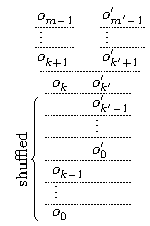
\includegraphics[width=2.7cm]{../figs/zipper-graph.pdf}
  };
\end{tikzpicture}
\end{align*}
The diagram on the right displays the structure of a zipper graph, assuming that $R$ and $R'$ have one operator per level.
The two subgraphs above the combined level correspond to $\widetilde{o}_{k+1}$ and $\widetilde{o}'_{k'+1}$ in $R_k$ and $R_{k'}'$.
\end{dfn}

\begin{thm}
\label{thm:frantz-mills-factorization}
\thmtitle{The Frantz-Mills factorization theorem}
\thmstatement{
$\displaystyle{
  RR'
=
  \sum_\pi
  (RR')_\pi^{k,k'}
}$
}
\thmproof{
}
\end{thm}



\begin{dfn}
\label{dfn:insertion-graph}
\thmtitle{Insertion graph}
\end{dfn}


%\begin{dfn}
%\thmtitle{Insertion graph}
%The graphs encountered in perturbation theory contain operators separated by resolvents.
%Two disconnected parts are termed \textit{separate} if no resolvent line crosses both.
%Vertical spaces between resolvent lines are termed \textit{levels}, which we number from %top to bottom for each separate part.
%A pair of resolvents with no intervening operators encloses an \textit{empty level}.
%Inserted brackets in the bracketing expansion produce separate and unlinked \textit{insertion graphs}.
%The empty level in the \textit{remainder} created by the insertion is the \textit{level of the insertion}.
%\end{dfn}



\end{document}